\chapter{PID tuning as a multi-objective optimization problem}
\label{chap:PIDMOOP}
%-----------------------------
\abstract{The \gls{pid} tuning problem stated in Chapter~\ref{chap:PIDControllerDesign} is solved using the \gls{ennc} methodology presented in Chapter~\ref{chap:Multi-objective}. The problem is solved using a \matlab{} script that can be found in the appendix of this chapter and also downloaded as a companion software. The result of this script is a set of files that define 2200 Pareto fronts with the optimal solutions of the problem of finding the tuning of \gls{2dof} \gls{pid} controller for \gls{soptd} plant families. Then two possible approaches are presented to interpret these results: first an attempt to find a tuning rule based on this data is presented. This approach was found to be very difficult to apply given the complexity of the data. The second approach is to use the data as a database and create a Graphical User Interface (GUI) to serve as the bridge between the user and the results. This GUI was encapsulated as a \matlab{} app and is also included as the companion software for this book.}
%-----------------------------
\section{Solution of the multiobjective optimization tuning}
\label{sec:SolMOOP}
When solving the \gls{moop} presented in Section~\eqref{sec:CostProbPID} for different normalized plants, one is able to find a family of Pareto fronts. With $L$ as the deadtime and $T$ as the lag time (also known as the constant time) and defining the normalized variable $\hat{s}=T s$, the time delay for the normalized plant, $\tau_0$, becomes:
\begin{equation}
\tau_0 = \frac{L}{T},
\label{eq:tauNorm}
\end{equation}
%
this yields the corresponding Pareto front for the normalized plant, which represents many possible combinations of lag time and deadtime. The gain of the plant is considered to be included in the controller gain for the sake of the normalization.

The problem at hand is to minimize $J_r(\bm{\theta})$, $J_{di}(\bm{\theta})$ and $J_{do}(\bm{\theta})$ simultaneously. In addition, the obtained parameters are constrained to always satisfy  $\gls{ms} \leq M_{s,max}$, where $M_{s,max}$ is the allowed limit of the Maximum Sensitivity. The combined cost function (vector of cost functions) then becomes:
%
\begin{equation}  %inclusión de ecuaciones
	\textbf{J}(\bm{\theta})=\left[J_{di}(\bm{\theta}), J_{do}(\bm{\theta}), J_{r}(\bm{\theta})\right]^T.
	\label{eq:Jtotal}
\end{equation}
%

With this cost function, the optimization problem is posed as:
%
\begin{equation}  %inclusión de ecuaciones
	\begin{gathered}
		\textbf{J}(\bm{\theta}^*) = \min_{\bm{\theta}} \textbf{J}(\bm{\theta}),\\
		\text{s.t.} \quad  M_s \leq M_{s,max}
	\end{gathered}
	\label{eq:probmooRepris}
\end{equation}
%
and the idea is to find a set of Pareto fronts for various cases of $\tau_{0}$. The steps that are required to find each one of the Pareto fronts are presented in Algorithm~\ref{alg:GenerateParetos3}. %
%
\begin{algorithm}[tb]
	\begin{algorithmic}
		\State $M_{svec} \gets [10,2,1.8,1.6,1.4]$
		\State $\tau_{0vec} \gets (0.1:0.1:2)$
		\State $a_{vec} \gets (0:0.1:1)$
		\ForAll{permutations of $M_s \in M_{svec}$, $\tau_0 \in \tau_{0vec}$ and $a \in a_{vec}$}
			\State Define the plant \gls{plan} with $\tau_{0}$ and $a$
			\State Find initial tuning  using uSORT2 method
			\State Create cost function $J(\theta) = [J_{di}(\theta, \gls{plan}, t),J_{do}(\theta, \gls{plan}, t),J_{r}(\theta, \gls{plan}, t) ]$
			\State Create constraint function $MCalc(\theta, \gls{plan}) \leq M_s$
			\State Apply \gls{ennc} method to find the Pareto front
			\State Apply Pareto filter
			\State Compute actual $M_s$ for each controller
			\State Save to file
		\EndFor
	\end{algorithmic}
\caption{Script for finding all Pareto fronts.}
\label{alg:GenerateParetos3}
\end{algorithm}
%
%
A Pareto front was found for each normalized plant with approximately 1000 points for each one. Using the steps of Algorithm~\ref{alg:GenerateParetos3}, a total of 220 different normalized plants were analyzed, as well as five different values of $M_{s,max}$, totaling to 1100 cases.

Notice that each of these points represent a different tuning (and since the optimization was done for \gls{2dof} controllers, each point has a different value for $\kappa_p$, $\tau_i$, $\tau_d$ and $\beta$), the total possible Pareto optimal \gls{pid} controllers found, reaches approximately 500 000 different controllers for all the totality of the plants and $M_{s,max}$. All these controller tunings can also be found in the companion software of this book as comma separated values files.

In regard to the robustness constraint, it has to be noticed that the constraint is of an inequality kind, that is:
\begin{equation*}
	M_s(\theta, \gls{plan}) \leq M_{s,max},
\end{equation*} 
in this particular case, the maximum sensitivity is set as $2.0$, $1.8$, $1.6$ or $1.4$. A maximum sensitivity of $M_{s,max} = 10.0$ was used as a way to relax the constraint in such a manner that practically the optimization was done without constraints with the advantage of being able to use the same script.

The function to compute the Pareto front with the \gls{ennc} method transforms the multiobjective cost function into a single function using the scalarization method presented in Section~\ref{sec:ENNC}. The function uses a standard optimization procedure\footnote{The function \texttt{fmincon} of the \matlab{} optimization toolbox was applied} to find each of the points of the Pareto. The \gls{ennc} function was based on the work of \citet{Houska2011} and \citet{Logist2012}, the Pareto filter used was as in \citet{Cao2020}.

A very important part of the computation is the implementation of the cost function. It is desirable to have a convex function to minimize, since a global minimum is most likely to be found. However, when using the \gls{iae} as a measure of the performance of the closed-loop response, the resulting cost function is not convex. In fact, the implementation of the cost function requires one to perform a simulation of the dynamic model and compute the integral of the absolute value of the error.

It is common to implement this cost function using \simulink, and in general it is a straightforward way to compute the cost function. However, it requires loading all the functionalities of \simulink{} with features that may not be used to compute the \gls{iae}. Consider now that to compute one single point of the Pareto entails using an optimization method with dozens of iterations and possibly hundreds of calls to the cost functions and each of these call functions necessitate \simulink{}. Remember that to solve the problem presented in this section, it is expected to find around 1000 points for each of the 1100 different cases. Potentially, to find all the Pareto fronts that are intended, millions of \simulink{} implementation of the cost function call may be needed. Considering this panorama, it is practically mandatory to find a faster implementation of the cost function.

In view of this and in order to solve the problem in \eqref{eq:probmooRepris} the computation of the \gls{iae} was implemented with a hybrid approach between \matlab{} and the C language with the aim to avoid the call to \simulink. Instead, the differential equations of the closed-loop response were solved using an implementation of the fourth order Runge--Kutta numerical method. The simulation was implemented in C with the API provided by \matlab. Using the \texttt{mex} instruction, the function is compiled and then called all the times needed. It was found that using this approach, the simulation time was reduced $97.7\%$ while the average error with respect to the simulation in \simulink{} was $9.118\times10^{-8}$. The \gls{iae} is computed later in a \matlab{} function with the results of the simulation. In all cases, a step input was used for all the sources of disturbance.

Finding all this data is time-consuming, even with the C implementation. It would be impractical to find the Pareto front every time it is needed, thus best practice would be to find the complete set of Pareto fronts once and save the results for later use.

However, there are two possible ways to utilize the data. On one hand, the data can be used to find a tuning rule that is as simple as possible that approximates the results of the optimizations. The other option is to create a software tool capable to access the files and interpolate the final tuning. In both cases, a way to incorporate the user preferences needs to be addressed.

In the following, these two possible routes are considered with two examples on how it may be done. First, an example of how to find a possible tuning rule using the data for dead-time dominated processes is presented. The obtained results are good, however, given the complexity of the data, the tuning rule turned out not to be as simple as desired. Later, a \gls{cad} program is presented that is capable of finding a controller tuning based on the idea of ``Maximum allowed degradation'' of the cost function. In short, this tool lets the user navigate into the Pareto front, without the need to visualize the Pareto, whilst letting the user to select the final tuning.

\section{Viability for tuning rules}
\label{sec:TuningRulesMOOP}
This section presents two examples on how to use the gathered data from the Pareto front in order to find a tuning rule.

The first example uses a reduced set of data where only $J_{di}$ and $J_{do}$ cost functions are considered and a \gls{pi} controller is tuned. The decision variable is the allowed degradation of the $J_{di}$ cost function. These results were first documented by \citet{ContrerasLeiva2015a}. 

The second example shows the results of a \gls{pid} controller tuning that takes into account all three proposed sources of disturbances ($J_{di}$, $J_{do}$ and $J_r$) for plants that are delay dominant. These results where first documented by \citet{Moya2017}.

\subsection{Tuning of a PI controller with two cost functions}
\label{sec:PI2FunMonica}
In this case, the Pareto front was conformed just by the cost functions $J_{di}$ and $J_{do}$ and with a simple first order model given by:
\begin{equation}
	P(s) = \frac{K e^{-Ls}}{Ts+1}.
\end{equation}

However, only \gls{pi} controllers were considered. The set of data is not equal to the data presented in Section~\ref{sec:SolMOOP}, instead it was found using the LCR scalarization \citep{Rojas2015b}, but the idea behind the tuning is the same.

In this case, only the feedback controller $C_y(s,\bm{\theta})$ of Figure~\ref{fig:Ch4controlador} is employed. After analyzing the data, it was found that one possible function that represents the variation of $\kappa_p$ with respect to the degradation variable $\alpha$ is given by:
\begin{equation}  %inclusión de ecuaciones
\kappa_p = a(\alpha) +b(\alpha)\tau_0^{c(\alpha)},
\label{ec:KpMonica}
\end{equation}
%
with parameters:
\begin{align*}
%
a(\alpha) &=  a_1 \alpha + a_2 \alpha^2,\\%
%\label{ec:a}\\
%
b(\alpha) &=  b_0  + b_1 \alpha,\\%
%\label{ec:b}\\
%
c(\alpha) &=  c_0  + c_1 \alpha^2.%
%\label{ec:c}
\end{align*}

For the case of the integral time, the proposed rule is given by:
\begin{equation}  %inclusión de ecuaciones
\tau_i = d(\alpha) +e(\alpha)\tau_0^{f(\alpha)},	\label{ec:TiMonica}\\
\end{equation}
%
where the parameters can be computed as:
\begin{align*}  %inclusión de ecuaciones
d(\alpha) &= d_0 + d_1 \alpha + d_2 \alpha^2,\\
%\label{ec:d}\\
%
e(\alpha) &= e_0 + e_1 \alpha,\\
%\label{ec:e}\\
%
f(\alpha) &= f_0 + f_2 \alpha^2.\\
%\label{ec:f}
\end{align*}

As it can be seen, to compute $\kappa_p$ and $\tau_i$, it is necessary to know 13 different constants. These constants are found using a curve fitting procedure that depends on the normalized deadtime and the maximum sensitivity $M_{s,max}$. The values found for $\kappa_p$ constants are presented in 
\begin{table}[tb]
	\caption{Constants associated with $\kappa_p$ in \eqref{ec:KpMonica}.} 
	\centering
	\begin{tabular}{@{}*{4}{m{2cm}}@{}}
		\toprule
		& $M_s\leq2$          & $M_s\leq1.8$   & $M_s\leq1.6$ \\
		\midrule
		\multicolumn{4}{c}{$0.1\leq\tau_0\leq0.5$}\\
		\midrule
		$a_1$  & $0.2887   $ 	  & $0.18960 $	   & $0.08484 $ \\
		$a_2$  & $-0.8579	$ 	  & $-0.3039 $	   & $-0.1811 $ \\
		$b_0$  & $0.6053	$     & $0.5356	 $	   & $0.4500  $ \\
		$b_1$  & $0.3205	$     & $0.1592  $	   & $0.1161  $ \\
		$c_0$  & $-0.9917	$ 	  & $-0.9928 $	   & $-0.9897 $ \\
		$c_1$  & $0.1341 	$  	  & $0.04427 $	   & $0.03272 $ \\
		\midrule
		\multicolumn{4}{c}{$0.6\leq\tau_0\leq2.0$}\\
		\midrule
		$a_1$  & $0.08305  $	& $0.001233 $	 & $0.003224$ \\
		$a_2$  & $-0.05774	$ 	& $-0.02813 $	 & $-0.01945$ \\
		$b_0$  & $0.8470	$ 	& $0.6964	$	 & $0.53560 $ \\
		$b_1$  & $-0.06829 $	& $0.07708 	$	 & $0.05128 $ \\
		$c_0$  & $-0.6934	$	& $-0.6921	$	 & $-0.7940 $ \\
		$c_1$  & $0 	    $   & $0 	    $    & $0       $ \\		
		\bottomrule
	\end{tabular}
	\label{tab:01Monica}
\end{table}
%
\begin{table}[tb]
	\caption{Constants associated with $\tau_i$ in \eqref{ec:TiMonica}.} 
	\centering
	\begin{tabular}{@{}*{4}{m{2cm}}@{}}
		\toprule
		&$M_s\leq2$     & $M_s\leq1.8$   & $M_s\leq1.6$ \\
		\midrule 
		\multicolumn{4}{c}{$0.1\leq\tau_0\leq0.4$}\\
		\midrule
		$d_0$  &$ 0  	   $    & $0 	    $    & $0       $\\
		$d_1$  &$ 1.3840  $    & $0.9996	$	 & $0.9685  $ \\
		$d_2$  &$ -0.4286 $	& $-0.07516 $	 & $-0.05125$ \\
		$e_0$  &$ 1.4440  $    & $1.3590 	$	 & $1.3110  $ \\
		$e_1$  &$ -1.179  $	& $-1.0500 	$	 & $-1.0970 $ \\
		$f_0$  &$ 0.6197  $    & $0.5474	$	 & $0.4775  $ \\
		$f_2$  &$ 0 	   $    & $0 	    $    & $0       $ \\
		\midrule
		\multicolumn{4}{c}{$0.5\leq\tau_0\leq2.0$}\\
		\midrule
		$d_0$  & $0.4483$ 	 	  & $0.5623$    &$0.6746 $ \\
		$d_1$  & $0.5070$ 	 	  & $0.3530$    &$0.3607 $ \\
		$d_2$  & $0 	$ 	      & $0 	   $    &$0      $ \\
		$e_0$  & $0.8717$		  & $0.6029$	&$0.3793 $ \\
		$e_1$  & $-0.418$	 	  & $-0.1828$	&$-0.2590$ \\
		$f_0$  & $0.6532$		  & $0.7480$	&$0.7055 $ \\
		$f_2$  & $0.2085$         & $0.0114$    &$0.4632 $ \\
		\bottomrule
	\end{tabular}
	\label{tab:02Monica}
\end{table}
Table~\ref{tab:01Monica} and those of $\tau_i$ are in Table~\ref{tab:02Monica}.

It is important to note that in order to find these equations, a series of curve fitting procedures were required. This is not a trivial task and even for a simple model like the one used in this example and a reduced controller, the quantity of computation needed is very high.

This is an example on how the Pareto front can be used as the basis to create models that allow extraction of the results without using the Pareto directly. Of course, the functions should be as close as possible to the values of the Pareto. In %
%
\begin{table}[t]
\caption{Approximation indexes for $\kappa_p$ in \eqref{ec:KpMonica}.}
	\centering
		\begin{tabular}{@{}*{3}{p{1.2cm}}@{}}
		\toprule
		 $M_s$     & $\tau_0$            & R-squared \\
    	\midrule
        $2.0$      & $\tau_0\leq0.5$   &$0.9982$	\\
        	       & $\tau_0\geq0.6$   &$0.9929$    \\
        $1.8$      & $\tau_0\leq0.5$   &$0.9994$	\\
	    	       & $\tau_0\geq0.6$   &$0.9945$    \\
	    $1.6$      & $\tau_0\leq0.5$   &$0.9996$	\\ 
	         	   & $\tau_0\geq0.6$   &$0.9971$	\\	
	   \bottomrule
	\end{tabular}
	\label{tab:cftoolkpMonica}
\end{table}
%
\begin{table}[t]
\caption{Approximation indexes for $\tau_i$ in \eqref{ec:TiMonica}.}
	\centering
		\begin{tabular}{@{}*{3}{p{1.2cm}}@{}}
		\toprule
		$M_s$		& $\tau_0$		& R-squared\\
  		\midrule
       $2.0$      & $\tau_0\leq0.4$      & $0.9925$ \\
       			  & $\tau_0\geq0.5$      & $0.9947$ \\
        $1.8$     & $\tau_0\leq0.4$      & $0.9978$	\\
                  & $\tau_0\geq0.5$      & $0.9986$ \\
        $1.6$     & $\tau_0\leq0.4$      & $0.9960$	\\
                  & $\tau_0\geq0.5$      & $0.9936$	\\	
		\bottomrule
	\end{tabular}
	\label{tab:cftoolTiMonica}
\end{table}
%
Table~\ref{tab:cftoolkpMonica} the mean R-squared value is presented for the case of the regression on the $\kappa_p$ variable and for the case of $\tau_i$ in Table~\ref{tab:cftoolTiMonica}. As it can be seen, the selected function and parameters fit the data well, which should give the user confidence that using \eqref{ec:KpMonica} and \eqref{ec:TiMonica} will most likely give Pareto optimal results and thus can be considered as an optimal tuning rule.

This tuning rule is comparable to other optimal tuning rules as in \citet{Murril1967} and  \citet{Alfaro2012a}, because in all cases, an integral cost function is optimized. In the case of the Murrill tuning \citep{Murril1967}, the \gls{iae} is minimized for disturbance rejection, while in the case of the uSORT method \citep{Alfaro2012a}, the disturbance rejection response is also minimized, but the maximum sensitivity is taken into account as a measure of robustness.

For these two methods, only the input disturbance is considered, while in the proposed method of this example, the user can vary the response between being optimal to the input disturbance or optimal to the output disturbance, giving more flexibility to the tuning. A controller was tuned with these three methods and compared in Table~\ref{tab:desemJdiMonica}.
%
\begin{table}[tb]
	\caption{Comparison of the performance of the closed-loop $J_{di}$.}
	\centering
	\begin{tabular}{@{}*{4}{p{2cm}}@{}}
		\toprule
		$\tau_0$   & Tuning        &IAE        & $M_s$ 	 \\
		\midrule
		$0.1$      & uSORT        &$0.0615$  &$2.0016$  \\
		$   $      & Murrill  &$0.0425$  &$3.8956$  \\
		$   $      & Proposed tuning            &$0.1081$  &$2.0399$  \\	
		$0.5$      & uSORT        &$0.7388$  &$2.0099$  \\				
		$   $      & Murrill  &$0.6186$  &$2.9757$  \\
		$   $      & Proposed tuning           &$0.8330$  &$1.7757$  \\
		$1.0$      & uSORT        &$1.6760$  &$2,0047$  \\				
		$   $      & Murrill  &$1.6710$  &$2.1831$  \\
		$   $      & Proposed tuning            &$1.5730$  &$2.0366$  \\		
		\bottomrule				
	\end{tabular}
	\label{tab:desemJdiMonica}
\end{table}
%
As it can be seen from this table, for $\tau_0 = 0.1$ and $\tau_0 = 0.5$, Murril presents the best performance, but in both cases, the value of $M_s$ is rather high, which is undesirable for real control loops. The method presented here gives results very similar to the ones obtained with uSORT, which is expected, since both methods minimize an integral cost function with $M_s$ as the robustness constraint. The advantage of the method shown in this example is that the user has an extra variable to fine tune the response.
%
\subsection{Tuning for a Three-objective PID controller}
\label{sec:Tuning3PID}
In this example, an \gls{soptd} plant is selected and represented by the normalized model:
\begin{equation}
	F(s) = \frac{e^{-\tau_{0} s}}{(s+1)(a s+1)}.
	\label{eq:Fs2ordenModeloChap7}
\end{equation}

For the next example, the variable $a$ takes values from $0$ to $1$ in $0.1$ steps, $\tau_0$ takes values from $1$ to $2$ in $0.1$ steps and the maximum sensitivity is constrained to $M_{s,max}=2$.

A curve fitting procedure was implemented to find useful equations for computing the value of $\kappa_p$, $\tau_i$, $\tau_d$ and $\beta$ as a function of $a$ and $\tau_0$ and a factor of degradation of the cost functions $J_{di}$.

Knowing the model of the plant, the values of the controller parameters can be computed without needing to perform all the optimizations, and the decision maker can also select the weight for each cost function in order to find a single set of parameters.

This idea of ``allowed degradation'' is now introduced. Considered that $J_{di}$ and $J_{do}$ are normalized as:
%
\begin{align}
\delta &= \frac{J_{di}(\theta)-J_{di, min}(\theta)}{J_{di,max}(\theta)-J_{di,min}(\theta)},\label{eq:delta}\\
\gamma &= \frac{J_{do}(\theta)-J_{do, min}(\theta)}{J_{do,max}(\theta)-J_{do,min}(\theta)},\label{eq:gamma}
\end{align}
%
such as both $0 \le \delta \le 1$ and $0 \le \gamma \le 1$. Then, these variables can be understood as the degradation of the function, considering the minimum value of the cost function as its optimal. Then a value of $\delta=1$ represents a degradation of 100\% of the $J_{di}$ cost function. It is important to notice that the Pareto front is constructed from three different cost functions. Therefore, if one selects the value of the allowed degradation for two functions (in this case, $\delta$ and $\gamma$), the logical step is to choose the lowest value of $J_r$ that complies with the maximum degradation of the other two functions. Then for example,  if $\delta=\gamma=1$, which means that the decision maker is willing to allow a complete degradation of $J_{di}$ and $J_{do}$, the resulting tuning is expected to represent the optimal tuning for servo control.

Now, it is important to understand that the ``degraded'' tuning, is also optimal in the Pareto sense, because all found tunings are optimal. Therefore, in these framework, a degraded tuning does not mean a ``bad'' tuning, it is just the result of a choice decision when selecting the desired controller. In all Pareto decisions, a compromise has to be made when selecting the ultimate solution.

The work done to find the tuning rules, summed up to almost two hundred and twenty regressions for all values of $a$ and $\tau_0$ in order to find the complete set of parameters $\bm{\theta}$.

After different heuristic tests, the regression analysis showed that a second order fit gave the best results for $\kappa_p$, $\tau_i$ and $\tau_d$,  while  a first order fit for $\beta$ was enough to model the variation of this parameter. 

The tuning rule for all controller parameters are proposed to be as:  
%
\begin{align}
\kappa_p &= p_{00}+p_{01}\cdot\gamma+p_{02}\cdot\delta\nonumber\\
&\quad + p_{03}\cdot\gamma^2+p_{04}\cdot\gamma\cdot \delta+p_{05}\cdot\delta^2,\label{E:eqkp}\\
%
\tau_i &= p_{10}+p_{11}\cdot\gamma+p_{12}\cdot\delta\nonumber\\
&\quad + p_{13}\cdot\gamma^2+p_{14}\cdot\gamma\cdot \delta+p_{15}\cdot\delta^2,\label{E:eqTi}\\
%
\tau_d &= p_{20}+p_{21}\cdot\gamma+p_{22}\cdot\delta\nonumber\\
&\quad+p_{23}\cdot\gamma^2+p_{24}\cdot\gamma\cdot \delta+p_{25}\cdot\delta^2,\label{E:eqTd}\\
%
\beta &=p_{30}+p_{31}\cdot\gamma+p_{32}\cdot\delta,\label{E:eqbeta}
\end{align}
%

The coefficients $p_{ij}$, where $i=\{0,1,2,3\}$ and $j=\{0,1,2,3,4,5\}$, depend on $a$ and $\tau_0$. The corresponding fits of $\kappa_p$, $\tau_i$, $\tau_d$ and $\beta$, are shown in Fig.~\ref{F:cftoolkp}. \ref{F:cftoolTi}, \ref{F:cftoolTd} and \ref{F:cftoolbeta} for $a=0.1$ and $\tau_{0}=1$.   % a second order surface was found to be the best fit for all eleven fits overall, as shown in figure \ref{F:firstfit}.
%
\begin{figure}[tb]
	\centering
	\includegraphics[width=\columnwidth]{kpfit2.png}
	\caption{Second order fit for $\kappa_p$ when $a=0.1$ and $\tau_{0}=1$}
	\label{F:cftoolkp}
\end{figure}
%
\begin{figure}[tb]
	\centering
	\includegraphics[width=\columnwidth]{Tifit2.png}
	\caption{Second order fit for $\tau_i$ when $a=0.1$ and $\tau_0=1$}
	\label{F:cftoolTi}
\end{figure}
%
\begin{figure}[tb]
	\centering
	\includegraphics[width=0.8\textwidth]{Tdfit2.png}
	\caption{Second order fit for $\tau_d$ when $a=0.1$ and $\tau_0=1$}
	\label{F:cftoolTd}
\end{figure}
%
\begin{figure}[tb]
	\centering
	\includegraphics[width=0.8\textwidth]{betafit2.png}
	\caption{First order fit for $\beta$ when $a=0.1$ and $\tau_0=1$}
	\label{F:cftoolbeta}
\end{figure}

However, there is a caveat. In those figures, the values that belong to the computed Pareto are shown as dots, while the corresponding regression is plotted as a 3D surface. It can be noticed that the domain of the regressions is larger than the actual results of the Pareto. Even though the fitting is good (around $R=0.9$), the regression represents interpolation and extrapolation from the real data. Therefore, it is important to check how well the regression works and to not exceed the limits where it yields good results.

Going back to the $p_{ij}$, it has to be noticed that the value of these parameters, depends on the model of the plant. Therefore, it is required to find another set of regressions over these parameters in terms of $a$ and $\tau_0$. Therefore, a curve fitting procedure is also required for each $p_{ij}$. As an example of these regressions, 
%
\begin{figure}[tb]
	\centering
	\includegraphics[width=0.8\textwidth]{./a00fit2.png}
	\caption{Second order fit for $p_{00}$ in $\kappa_p$}
	\label{F:coeff}
\end{figure}
%
Fig.~\ref{F:coeff} shows the result for $p_{00}$ parameter as a function of $a$ and $\tau_0$. The selected fit for every coefficient in the range of $1\leq \tau_0 \leq2$, was also a second-order polynomial. The equation that is considered has the form:
%
\begin{equation}
p_{ij} = b_{j0}+b_{j1}a+b_{j2} \tau_0+b_{j3}a^2+b_{j4}a \tau_0+b_{j5}\tau_0^2 .
\label{E:coeff}
\end{equation}

Another two hundred and twenty regressions were made for each $p_{ij}$. The results for every coefficient are shown in Table~\ref{T:T1} for $\kappa_p$, Table~\ref{T:ti} for the integral time, Table~\ref{T:td} for the derivative time and Table~\ref{T:beta} for $\beta$.

% Please add the following required packages to your document preamble:
% \usepackage{multirow}
%\begin{table}
%\centering
%\caption{Parameters for $\kappa_p$.}
%\label{T:T1}
%\begin{tabular}{|c|l|l|}
%\hline
%\multicolumn{3}{|c|}{$\kappa_p$ coefficients}           \\ \hline
%$p_{ij}$                  & \multicolumn{2}{c|}{$b_{ik}$} \\ \hline
%\multirow{6}{*}{$p_{00}$} & $b_{00}$      & 1.8203        \\ \cline{2-3} 
%                     & $b_{01}$      & 0.12765       \\ \cline{2-3} 
%                     & $b_{02}$      & -1.0484       \\ \cline{2-3} 
%                     & $b_{03}$      & 0.27085       \\ \cline{2-3} 
%                     & $b_{04}$      & -0.15141      \\ \cline{2-3} 
%                     & $b_{05}$      & 0.25505       \\ \hline
%\multirow{6}{*}{$p_{01}$} & $b_{10}$      & 0.32832       \\ \cline{2-3} 
%                     & $b_{11}$      & 0.22439       \\ \cline{2-3} 
%                     & $b_{12}$      & -0.26761      \\ \cline{2-3} 
%                     & $b_{13}$      & -0.022374     \\ \cline{2-3} 
%                     & $b_{14}$      & -0.068708     \\ \cline{2-3} 
%                     & $b_{15}$      & 0.076273      \\ \hline
%\multirow{6}{*}{$p_{02}$} & $b_{20}$      & 0.29122       \\ \cline{2-3} 
%                     & $b_{21}$      & -0.12878      \\ \cline{2-3} 
%                     & $b_{22}$      & -0.25003      \\ \cline{2-3} 
%                     & $b_{23}$      & 0.10461       \\ \cline{2-3} 
%                     & $b_{24}$      & 0.0048329     \\ \cline{2-3} 
%                     & $b_{25}$      & 0.059478      \\ \hline
%\multirow{6}{*}{$p_{03}$} & $b_{30}$      & 0.042733      \\ \cline{2-3} 
%                     & $b_{31}$      & -0.52048      \\ \cline{2-3} 
%                     & $b_{32}$      & -0.25437      \\ \cline{2-3} 
%                     & $b_{33}$      & 0.47345       \\ \cline{2-3} 
%                     & $b_{34}$      & -0.11069      \\ \cline{2-3} 
%                     & $b_{35}$      & 0.078691      \\ \hline
%\multirow{6}{*}{$p_{04}$} & $b_{40}$      & -0.077455     \\ \cline{2-3} 
%                     & $b_{41}$      & 0.61083       \\ \cline{2-3} 
%                     & $b_{42}$      & 0.24951       \\ \cline{2-3} 
%                     & $b_{43}$      & -0.60316      \\ \cline{2-3} 
%                     & $b_{44}$      & 0.19685       \\ \cline{2-3} 
%                     & $b_{45}$      & -0.071314     \\ \hline
%\multirow{6}{*}{$p_{05}$} & $b_{50}$      & -0.41226      \\ \cline{2-3} 
%                     & $b_{51}$      & -0.24733      \\ \cline{2-3} 
%                     & $b_{52}$      & 0.29554       \\ \cline{2-3} 
%                     & $b_{53}$      & 0.080236      \\ \cline{2-3} 
%                     & $b_{54}$      & 0.013411      \\ \cline{2-3} 
%                     & $b_{55}$      & -0.091089     \\ \hline
%\end{tabular}
%\end{table}
%
\begin{table}[tb]
	\centering
	\caption{Coefficients for $\kappa_p$.}
	\label{T:T1}
	\begin{tabular}{@{}cll|cll@{}}
		\hline
		%\multicolumn{6}{c}{$\kappa_p$ coefficients}           \\ \hline
		$p_{ij}$                  & \multicolumn{2}{c}{$b_{ik}$} & $p_{ij}$ & \multicolumn{2}{c}{$b_{ik}$}\\
		\hline
		\multirow{6}{*}{$p_{00}$} & $b_{00}$  & $1.820$ &   \multirow{6}{*}{$p_{01}$} & $b_{10}$ & $0.328$ \\ % \cline{2-3} \cline{5-6}
		& $b_{01}$      & $0.128$   &  	& $b_{11}$      & $0.224$ \\ % \cline{2-3} \cline{5-6}
		& $b_{02}$      & $-1.048$   &	& $b_{12}$      & $-0.268$ \\ % \cline{2-3} \cline{5-6}
		& $b_{03}$      & $0.270$   &	& $b_{13}$      & $-0.022$ \\ % \cline{2-3} \cline{5-6}
		& $b_{04}$      & $-0.151$  & 	& $b_{14}$      & $-0.069$  \\ % \cline{2-3} \cline{5-6}
		& $b_{05}$      & $0.255$   &	& $b_{15}$      & $0.076$    \\ \hline
		%
		\multirow{6}{*}{$p_{02}$} & $b_{20}$  & $0.291$	& \multirow{6}{*}{$p_{03}$} & $b_{30}$ & $0.043$ \\ % \cline{2-3} \cline{5-6}
		& $b_{21}$      & $-0.129$   & & $b_{31}$      & $-0.520$  \\ % \cline{2-3} \cline{5-6}
		& $b_{22}$      & $-0.250$   & & $b_{32}$      & $-0.254$  \\ % \cline{2-3} \cline{5-6}
		& $b_{23}$      & $0.105$    & & $b_{33}$      & $0.473$   \\ % \cline{2-3} \cline{5-6}
		& $b_{24}$      & $0.005$  & & $b_{34}$      & $-0.111$  \\ % \cline{2-3} \cline{5-6}
		& $b_{25}$      & $0.059$   & & $b_{35}$      & $0.079$  \\ \hline
		%
		\multirow{6}{*}{$p_{04}$} & $b_{40}$      & $-0.077$  & \multirow{6}{*}{$p_{05}$} & $b_{50}$      & $-0.412$   \\ %\cline{2-3} \cline{5-6}
		& $b_{41}$      & $0.611$     &  & $b_{51}$      & $-0.247$\\ %\cline{2-3} \cline{5-6}
		& $b_{42}$      & $0.249$     &  & $b_{52}$      & $0.296$\\ % \cline{2-3} \cline{5-6}
		& $b_{43}$      & $-0.603$    &  & $b_{53}$      & $0.080$\\ %\cline{2-3} \cline{5-6}
		& $b_{44}$      & $0.197$     &  & $b_{54}$      & $0.013$\\ % \cline{2-3} \cline{5-6}
		& $b_{45}$      & $-0.071$   &  & $b_{55}$      & $-0.091$\\
		\hline
	\end{tabular}
\end{table}
%
\begin{table}[tb]
	\centering
	\caption{Coefficients for $\tau_i$.}
	\label{T:ti}
	\begin{tabular}{@{}cll|cll@{}}
		\hline
		%\multicolumn{6}{c}{$\kappa_p$ coefficients}           \\ \hline
		$p_{ij}$                  & \multicolumn{2}{c}{$b_{ik}$} & $p_{ij}$ & \multicolumn{2}{c}{$b_{ik}$}\\
		\hline
		\multirow{6}{*}{$p_{10}$} & $b_{00}$  & $0.591$
		&   \multirow{6}{*}{$p_{11}$} & $b_{10}$ & $-0.408$
		\\ % \cline{2-3} \cline{5-6}
		& $b_{01}$      & $0.559$   &  	& $b_{11}$      & $0.640$ \\ % \cline{2-3} \cline{5-6}
		& $b_{02}$      & $0.545$   &	& $b_{12}$      & $0.855$ \\ % \cline{2-3} \cline{5-6}
		& $b_{03}$      & $0.017$   &	& $b_{13}$      & $-0.238$ \\ % \cline{2-3} \cline{5-6}
		& $b_{04}$      & $0.045$  & 	& $b_{14}$      & $-0.0024$  \\ % \cline{2-3} \cline{5-6}
		& $b_{05}$      & $-0.028$   &	& $b_{15}$      & $-0.193$    \\ \hline
		%
		\multirow{6}{*}{$p_{12}$} & $b_{20}$  & $1.718$
		& \multirow{6}{*}{$p_{13}$} & $b_{30}$ & $1.297$ \\ % \cline{2-3} \cline{5-6}
		& $b_{21}$      & $0.652$   & & $b_{31}$      & $-0.423$  \\ % \cline{2-3} \cline{5-6}
		& $b_{22}$      & $-1.160$   & & $b_{32}$      & $-2.095$  \\ % \cline{2-3} \cline{5-6}
		& $b_{23}$      & $-0.855$    & & $b_{33}$      & $1.226$   \\ % \cline{2-3} \cline{5-6}
		& $b_{24}$      & $-0.719$  & & $b_{34}$      & $-1.041$  \\ % \cline{2-3} \cline{5-6}
		& $b_{25}$      & $0.363$   & & $b_{35}$      & $0.649$  \\ \hline
		%
		\multirow{6}{*}{$p_{14}$} & $b_{40}$      & $-0.077$  & \multirow{6}{*}{$p_{15}$} & $b_{50}$      & $-1.346$   \\ %\cline{2-3} \cline{5-6}
		& $b_{41}$      & $0.621$     &  & $b_{51}$      & $-1.148$\\ %\cline{2-3} \cline{5-6}
		& $b_{42}$      & $0.277$     &  & $b_{52}$      & $1.224$\\ % \cline{2-3} \cline{5-6}
		& $b_{43}$      & $-1.193$    &  & $b_{53}$      & $-0.218$\\ %\cline{2-3} \cline{5-6}
		& $b_{44}$      & $1.030$     &  & $b_{54}$      & $0.512$\\ % \cline{2-3} \cline{5-6}
		& $b_{45}$      & $-0.025$   &  & $b_{55}$      & $-0.572$\\
		\hline
	\end{tabular}
\end{table}
%
\begin{table}[tb]
	\centering
	\caption{Coefficients for $\tau_d$.}
	\label{T:td}
	\begin{tabular}{@{}cll|cll@{}}
		\hline
		%\multicolumn{6}{c}{$\kappa_p$ coefficients}           \\ \hline
		$p_{ij}$                  & \multicolumn{2}{c}{$b_{ik}$} & $p_{ij}$ & \multicolumn{2}{c}{$b_{ik}$}\\
		\hline
		\multirow{6}{*}{$p_{20}$} & $b_{00}$  & $0.111$
		&   \multirow{6}{*}{$p_{21}$} & $b_{10}$ & $-0.0076$
		\\ % \cline{2-3} \cline{5-6}
		& $b_{01}$      & $0.450$   &  	& $b_{11}$      & $-0.163$ \\ % \cline{2-3} \cline{5-6}
		& $b_{02}$      & $0.274$   &	& $b_{12}$      & $-0.212$ \\ % \cline{2-3} \cline{5-6}
		& $b_{03}$      & $-0.025$   &	& $b_{13}$      & $0.154$ \\ % \cline{2-3} \cline{5-6}
		& $b_{04}$      & $-0.069$  & 	& $b_{14}$      & $-0.074$  \\ % \cline{2-3} \cline{5-6}
		& $b_{05}$      & $0.003$   &	& $b_{15}$      & $0.0026$    \\ \hline
		%
		\multirow{6}{*}{$p_{22}$} & $b_{20}$  & $-0.238$	& \multirow{6}{*}{$p_{23}$} & $b_{30}$ & $-0.237$ \\ % \cline{2-3} \cline{5-6}
		& $b_{21}$      & $0.105$   & & $b_{31}$      & $-0.938$  \\ % \cline{2-3} \cline{5-6}
		& $b_{22}$      & $-0.016$   & & $b_{32}$      & $1.121$  \\ % \cline{2-3} \cline{5-6}
		& $b_{23}$      & $-0.234$    & & $b_{33}$      & $0.496$   \\ % \cline{2-3} \cline{5-6}
		& $b_{24}$      & $0.094$  & & $b_{34}$      & $0.331$  \\ % \cline{2-3} \cline{5-6}
		& $b_{25}$      & $-0.0254$   & & $b_{35}$      & $-0.641$  \\ \hline
		%
		\multirow{6}{*}{$p_{24}$} & $b_{40}$      & $0.379$  & \multirow{6}{*}{$p_{25}$} & $b_{50}$      & $-0.224$   \\ %\cline{2-3} \cline{5-6}
		& $b_{41}$      & $0.908$     &  & $b_{51}$      & $0.109$\\ %\cline{2-3} \cline{5-6}
		& $b_{42}$      & $-1.330$     &  & $b_{52}$      & $0.805$\\ % \cline{2-3} \cline{5-6}
		& $b_{43}$      & $-1.203$    &  & $b_{53}$      & $0.669$\\ %\cline{2-3} \cline{5-6}
		& $b_{44}$      & $0.215$     &  & $b_{54}$      & $-0.527$\\ % \cline{2-3} \cline{5-6}
		& $b_{45}$      & $0.683$   &  & $b_{55}$      & $-0.112$\\
		\hline
	\end{tabular}
\end{table}
%
\begin{table}[tb]
	\centering
	\caption{Coefficients for $\beta$.}
	\label{T:beta}
	\begin{tabular}{@{}cll}
		\hline
		%\multicolumn{6}{c}{$\kappa_p$ coefficients}           \\ \hline
		$p_{ij}$                  & \multicolumn{2}{c}{$b_{ik}$}  \\
		\hline
		\multirow{6}{*}{$p_{30}$} & $b_{00}$  & $0.538$
		
		\\ % \cline{2-3} \cline{5-6}
		& $b_{01}$      & $0.023$     \\ % \cline{2-3} \cline{5-6}
		& $b_{02}$      & $0.179$   	\\ % \cline{2-3} \cline{5-6}
		& $b_{03}$      & $-0.114$    \\ % \cline{2-3} \cline{5-6}
		& $b_{04}$      & $0.047$   	  \\ % \cline{2-3} \cline{5-6}
		& $b_{05}$      & $-0.034$   \\ \hline
		%
		\multirow{6}{*}{$p_{31}$} & $b_{10}$  & -0.152
		\\ % \cline{2-3} \cline{5-6}
		& $b_{11}$      & $0.065$    \\ % \cline{2-3} \cline{5-6}
		& $b_{12}$      & $0.277$      \\ % \cline{2-3} \cline{5-6}
		& $b_{13}$      & $0.017$      \\ % \cline{2-3} \cline{5-6}
		& $b_{14}$      & $-0.052$   \\ % \cline{2-3} \cline{5-6}
		& $b_{15}$      & $-0.082$     \\ \hline
		%
		
		\multirow{6}{*}{$p_{32}$} & $b_{20}$  & 0.585
		\\ % \cline{2-3} \cline{5-6}
		& $b_{21}$      & $-0.082$    \\ % \cline{2-3} \cline{5-6}
		& $b_{22}$      & $-0.280$      \\ % \cline{2-3} \cline{5-6}
		& $b_{23}$      & $0.116$      \\ % \cline{2-3} \cline{5-6}
		& $b_{24}$      & $0.011$   \\ % \cline{2-3} \cline{5-6}
		& $b_{25}$      & $0.044$     \\ \hline
		%	
	\end{tabular}
\end{table}
%
\subsubsection{Comparison of regression against Pareto data}
%
To compare the results from the tuning rule, some simulations were done to compare the original data against the results. The plant model is: 

\begin{equation}
P_1(s) = \frac{e^{-1.5\hat{s}}}{(\hat{s}+1)(0.5\hat{s}+1)}
\label{E:P1}
\end{equation}

Where $K=1$, $T=1$~s, $L=1.5$~s and $a = 0.5$. Table \ref{T:comparison} compares the results of the optimization against the results of using the proposed tuning rule. Arbitrarily, the values for $\delta$ and $\gamma$ were chosen as $\delta=1$ and $\gamma=1$. 
%
\begin{table}[tb]
	\centering
	\caption{Result comparative of the Pareto data against the fitted data, with $\delta = 1$ and $\gamma = 1$.}
	\label{T:comparison}
	\begin{tabular}{@{}K{0.25\columnwidth} K{0.25\columnwidth} K{0.25\columnwidth}@{}}
		\toprule
		$\bm{\theta}$ and cost functions & From Pareto & From Tuning rule\\
		\midrule
		$\kappa_p$	& $0.810$	& $0.793$ \\
		$\tau_i$	& $2.176$~s	& $2.113$~s	\\
		$\tau_d$	& $0.644$~s	& $0.720$~s \\
		$\beta$		& $1.000$	& $1.000$ \\
		$J_r$		& $2.689$ 	& $2.691$ \\
		$J_{di}$ 	& $2.687$ 	& $2.673$ \\
		$J_{do}$	& $2.689$	& $2.691$ \\
		$M_s$		& $1.9174$	& $1.9449$\\
		\bottomrule
	\end{tabular}
\end{table} 

In Table~\ref{T:comparison}, it can be seen that the results obtained from the  tuning rule are close to those obtained directly from the Pareto. Plots for each method were drawn as shown in Fig.~\ref{F:firstsim}.
%%%ESTA FIGURA HAY QUE CENTRARLA MEJOR
%
\begin{figure}[tb]
	\centering
	\includegraphics[width=\columnwidth]{servo2.png}
	\caption{Servo response for the Pareto results found with the \gls{nnc} method and the tuning results.}
	\label{F:firstsim}
\end{figure}
%
The control signal for a reference step response is shown in Figure~\ref{F:u1} while the comparison for an input-disturbance is presented in Figure~\ref{F:di1} and for the output disturbance is in Figure~\ref{F:do1}. 
%
\begin{figure}[tb]
	\centering
	\includegraphics[width=\columnwidth]{u2.png}
	\caption{Comparison of the control action  signal for a setpoint step change using the data from the Pareto found with the \gls{ennc} method and the tuning rule.}
	\label{F:u1}
\end{figure}
%
\begin{figure}[tb]
	\centering
	\includegraphics[width=\columnwidth]{di2.png}
	\caption{Step input disturbance response for tuning from Pareto (\gls{ennc} method) and regressions results.}
	\label{F:di1}
\end{figure}
%
\begin{figure}[tb]
	\centering
	\includegraphics[width=\columnwidth]{do2.png}
	\caption{Step output disturbance response for \gls{ennc} results and regressions results.}
	\label{F:do1}
\end{figure}
%
The figures show the \gls{iae} between both signals as a measure of how good the tuning rule approximates the optimization. As it can be seen, the responses are almost identical, showing that this methodology is feasible.

The tuning rule is also used for the extreme cases of $\tau_0$, that is, $\tau_0=1$ and $\tau_0=2$, using the following models:
%
\begin{equation}
P_F(\hat{s}) = \frac{e^{-\hat{s}}}{(\hat{s}+1)(0.5\hat{s}+1)},
\label{E:p2}
\end{equation}
%
\begin{equation}
P_S(\hat{s}) = \frac{e^{-2\hat{s}}}{(\hat{s}+1)(0.5\hat{s}+1)},
\label{E:p3}
\end{equation}
%
where $P_F(\hat{s})$ and $P_S(\hat{s})$ stand for the minimum and maximum  dead time considered in this study, respectively.

The allowed degradation was set to $\delta = 0.5$ and $\gamma = 0.5$. As before, one would expect to have the best servo response that complies with the allowed degradation. The comparison between the Pareto optimizations and the tuning rule for $P_F$ and $P_S$ are shown in Table~\ref{T:T2} and Table~\ref{T:T3} respectively.
%
\begin{table}[tb]
	\centering
	\caption{Results for $J_{di}$, $J_{do}$ and $J_{r}$, using $\delta = 0.5$ and $\gamma = 0.5$ for $P_F(s)$.}
	\label{T:T2}
	\begin{tabular}{@{}K{0.2\columnwidth} K{0.2\columnwidth} K{0.2\columnwidth} K{0.2\columnwidth}@{}}
		\toprule
		$\bm{\theta}$ and IAE & From tuning rule & From Pareto & Difference (\%)\\
		\midrule
		$\kappa_p$	& $1.150$ 	& $1.120$ & $2.67$\\
		$\tau_i$ 	& $1.987$ s & $1.900$ s & $4.58$\\
		$\tau_d$ 	& $0.425$ s & $0.495$ s & $-14.14$\\
		$\beta$ 	& $0.887$ 	& $0.889$ & $-0.23$\\
		$J_r$ 		& $1.955$ 	& $2.1446$ & $8.84$\\
		$J_{di}$ 	& $1.729$ 	& $1.6947$ & $2.02$\\
		$J_{do}$ 	& $1.874$ 	& $1.803$ & $3.94$\\
		$M_s$		& $2.024$	& $2.013$ & $0.55$\\
		\bottomrule
	\end{tabular}
\end{table} 
%
\begin{table}[tb]
	\centering
	\caption{Results for $J_{di}$, $J_{do}$ and $J_{r}$, using $\delta = 0.5$ and $\gamma = 0.5$ for $P_S(s)$.}
	\label{T:T3}
	\begin{tabular}{@{}K{0.2\columnwidth} K{0.2\columnwidth} K{0.2\columnwidth} K{0.2\columnwidth}@{}}
		\toprule
		$\bm{\theta}$ and IAE & From tuning rule & From Pareto & Difference (\%)\\
		\midrule
		$\kappa_p$	& $0.742$	& $0.744$	& $-0.270$\\
		$\tau_i$ 	& $2.345$ s	& $2.264$	& $3.578$\\
		$\tau_d$ 	& $0.629$ s	& $0.712$	& $11.657$\\
		$\beta$ 	& $0.919$	& $0.927$	& $-0.863$\\
		$J_r$ 		& $3.360$	& $3.662$	& $-8.247$\\
		$J_{di}$ 	& $3.162$	& $3.065$	& $3.165$\\
		$J_{do}$ 	& $3.237$	& $3.158$	& $2.502$\\
		$M_s$		& $1.976$	& $2.000$	& $-0.012$\\
		\bottomrule
	\end{tabular}
\end{table}

It is clear that the tuning rule is able to produce near Pareto-optimal controllers, in both cases the maximum error is in $\tau_d$.

One of the interesting features is that the decision maker is able to choose the final solution by given a suitable value to $\delta$ and $\gamma$ as they consider appropriate. Since the data used to find the tuning rule has been constrained to have a maximum sensitivity of $M_s =2.0$, it is expected to have a stable closed-loop. Another interesting characteristic of this tuning rule is its ability to select the appropriate parameters taking into account three different sources of disturbances, unlike other \gls{pid} tuning rules.

From Table~\ref{T:T2} and Table~\ref{T:T3}, it can be deduced that the tuning rule finds a controller that has a better servo response than using the data directly, but compromises the response to the input and output disturbance rejection.

\subsection{Comments on creating tuning rules from Pareto fronts}
\label{sec:TuningRules}
It is clear that it is feasible to find tuning rules from Pareto fronts as exemplified above. However, there are several points that need to be addressed:
\begin{itemize}
	\item The tuning rule was intended to be as simple as possible. However, it needed 126 coefficients to find the four parameters of the controller. Compared with other tuning rules such as the ones that can be found in \citet{odwyer2006}, this tuning rule is complex.
	%
	\item The idea of the degradation factor is interesting and directly related to the Pareto front, however, it is not as intuitive as setting something more measurable, as the time constant of the closed-loop system, for example.
	%
	\item The tuning rule is restricted to values of $1 \leq \tau_0 \leq 2$. The data for other values of $\tau_0$ exist, in fact, the reader can download the complete set of data from the companion software for this book. However, the complexity of the data made it unfeasible to find a good simple tuning rule for all possible values of $\tau_0$.
	%
	\item The tuning rule is also restricted to \gls{pid} controllers. But it is very common to use \gls{pi} controllers in the industry. However, it is not possible to just discard the derivative time from the obtained tuning.
	%
	\item The data obtained from the optimizations are constrained to have certain Maximum Sensitivity $M_{s,max}$. However, the presented rule takes into account only the value of $M_s = 2$. In order to have tuning rules for other values of $M_{s,max}$, possibly another set of 126 coefficients needs to be found for each desired value, which requires a lot of effort that may be not worth it.
\end{itemize}

All these points raise an important question, is it useful to find tuning rules that become too cumbersome for setting a \gls{pid} controller? The literature on \gls{pid} tuning generally shows simple tuning rules that need only a few decision parameters, for example \citet{Skogestad2003} need only the model of the plant and a desired time constant, or even no decision parameters, since they minimize a single cost function as in the MoReRT tuning rule \citep{Alfaro2016}.

However, using the multiobjective approach presented here, the relationships between the controller gains, the tuning parameters and the model parameters become so complex, that a simple tuning rule that compasses all cases is impossible to find.

In this case, a more direct approach may be better suited for the task of finding the best controller tuning. It is true that the Pareto front is not the final solution for the tuning problem, however only a selection is needed to ultimately find the desired solution. Therefore, a \textit{database} approach may be more sensible to the task at hand. This option is explored in the next section.
%
\section{Database approach for the final tuning}
\label{sec:DatabaseMOOP}
%
The information of the Pareto front is very valuable, each point represents an optimal controller tuning that also complies with the robustness criterion. However, without any guidance on how to choose the final tuning, the data is ultimately useless. The idea of using the Pareto as the basis for a tuning rule was explored in Section~\ref{sec:TuningRulesMOOP} for two degrees of freedom \gls{pid} controllers taking into account three different sources of disturbances and a robustness constraint for a \gls{soptd} plant. However it was found that a simple rule is very difficult to find, given the complexity of the relationship between the different parameters. For simpler cases, it may be possible to find suitable tuning rules, as in Section~\ref{sec:PI2FunMonica}, but for a more realistic case, the final tuning becomes cumbersome.

In this scenario, the other approach to take advantage of the information in the Pareto is to actually use the data directly. Visualizing the Pareto is also a difficult task, especially for more than two cost functions. Therefore, the approach that is presented here is to use a \gls{cad} that allows the user to select the desired closed-loop performance according to their needs without the need to plot the front.

The proposed \gls{cad} tool that accompanies this book is named MOOTuning, and is available as a \matlab{} app. A screenshot of the tool is presented in 
\begin{figure}[tb]
	\centering
	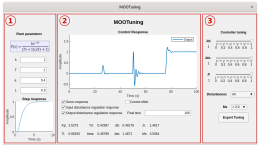
\includegraphics[width=\columnwidth]{Ch6MOOTuningParts}
	\caption{Interface of MOOTuning for PID parameter selection.}
	\label{fig:Ch6MOOTuningParts}
\end{figure}
Figure~\ref{fig:Ch6MOOTuningParts}. It has three main components:
\begin{enumerate}
	\item Plant parameters input section
	\item Results section
	\item Tuning section
\end{enumerate}
%
The plant parameters input section is used to enter the parameters of the model of the plant. The expected model is an \gls{soptd}, but the value of $a$ can be set to zero, giving the option to also have a \gls{foptd} model. However, it is necessary to have a normalized time delay larger than $0.1$. The tool warns the user when an invalid value is entered, for example a negative time constant. When any of these parameters are changed, the step response plot at the bottom is automatically updated.

The second section shows the user the results of the selected tuning. The main component is a figure where the closed-loop response is plotted for the selected sources of disturbance: \textit{Servo response} is the closed-loop response to a setpoint step change, \textit{Input disturbance regulation response} plots the closed-loop response to a step change at the input of the plant and \textit{Output disturbance regulation response} plots the closed-loop response to  step change at the output of the plant. The control effort can be plotted in the same graph as well.

At the bottom of the second section, the results of the controller parameters, the value of the cost function and the value of the maximum sensitivity are presented with the given tuning. These are updated every time the user makes a change in the third section of the tool.

The last section of the tool is the Tuning section. Here, the user is presented with a series of ``decision choices'' that define which of the points of the front are selected as the final tuning. The sliders at the top represent the \textit{allowed degradation} of the function with respect to the optimal point. A value of zero means that the lowest value of the cost function is desired, while a value of 1 represents that the function can have any value (even its maximum value).

The tool selects the function with the lowest allowed degradation as the main cost function. Then, it searches for a set of parameters that comply with all the degradation limits set by the user, which also has the lowest possible value of the main function. As it can be seen, this tool lets the user select the desired value from the Pareto without the need to plot the front.

The user has also the ability to select if all the cost functions need to be used for the tuning, or if only the input disturbance and the setpoint changes are utilized. Finally, the user can select different values of Maximum Sensitivity to set the robustness of the closed-loop system. The \textit{Export Tuning} button lets the user copy the values of the tuning and export them as a structure to the \matlab{} workspace.

Of course, it may be possible that the user selects a set of values for $J_{di}$, $J_{do}$ and $J_r$ that do not correspond to a Pareto point. In that case, the tool shows a window indicating that the current selection is not feasible. This window is shown in %
%
\begin{figure}[tb]
	\centering
	\includegraphics[width=\columnwidth]{Ch6MOOTuningError}
	\caption{Error raised if the desired point lies outside the Pareto front.}
	\label{fig:Ch6MOOTuningError}
\end{figure}
%
Figure~\ref{fig:Ch6MOOTuningError}. The user then needs to relax the allowed degradation of the cost function (i.e. increase the allowed degradation of one of the functions) to be able to find the appropriate tuning. Once the user is satisfied with the design, the tuning can be exported to the \matlab{} workspace and the figure can be saved using the standard \matlab{} methods\footnote{The tool was created using \matlab{} 2020a, earlier versions may not work as expected.}.

\subsection{Example using MOOTuning}
\label{sec:MOOTuningExample}
In the following, a typical workflow example is presented using the proposed tool. Suppose that the model of the plant to be controlled is given by:
\begin{equation}
	H(s) = \frac{0.6 e^{-5s}}{(10 s + 1)(2 s +1)}.
	\label{eq:ModeloEjemploMOO}
\end{equation}

From this transfer function, it can be seen that the parameters are given by $k=0.6$, $T=10$, $L=5$ and $a = 0.2$. The first step then consists of introducing these parameters into the tool, as shown in %
\begin{figure}[tb]
	\centering
	\includegraphics[scale=0.5]{Ch6MOOTuningExample01}
	\caption{Input of the parameters of the model into MOOTuning.}
	\label{fig:Ch6MOOTuningExample01}
\end{figure}
%
Figure~\ref{fig:Ch6MOOTuningExample01}. Every time a parameter is introduced, the tool updates the step response at the bottom of the screen. In this case, it can be seen that the plant takes approximately 50 seconds to reach a steady state. It should be noted that the tuning of the controller is not going to be updated until the allowed degradation of any functions is changed.

For this particular example, only two cost functions are going to be considered ($J_{di}$ and $J_r$) with the option of $M_s > 2.0$. Originally, the allowed degradation is one for both functions, which means that the response presented has the lowest \gls{iae} for servo response without any constraint on the input disturbance response. This initial closed-loop response is as presented in
%
\begin{figure}[tb]
	\centering
	\includegraphics[width=0.5\columnwidth]{Ch6MOOTuningExample02}
	\caption{Initial closed-loop response.}
	\label{fig:Ch6MOOTuningExample02}
\end{figure}
%
Figure~\ref{fig:Ch6MOOTuningExample02}. The response to an input disturbance and to a change in the setpoint is presented in the Tool. However, it can be seen that 100 seconds is not enough to see the complete response. Within a 200 second time window, the closed-loop response is given as presented in %
\begin{figure}
	\centering
	\includegraphics[width=\columnwidth]{Ch6MOOTuningExample03}
	\caption{Closed-loop response with a \SI{200}{\second} time window.}
	\label{fig:Ch6MOOTuningExample03}
\end{figure}
%
Figure~\ref{fig:Ch6MOOTuningExample03}.

As it can be seen, the disturbance rejection response is rather slow, and the servo response is appropriate. However, it is possible to find a compromise between both. Assume that a degradation of 20\% in the servo response can be tolerated. The tool can help to answer which is the best disturbance rejection response that can be achieved with this constraint. After trying different values, it was found that the best disturbance rejection response that can be achieved whilst simultaneously having a servo response with a degradation no greater than 20\% from its optimal value, has an allowed degradation of $32.6\%$ for $J_{di}$.%
%
\begin{table}[tb]
	\centering
	\begin{tabular}{cccc}
		\toprule
		Case & $J_{di}$ & $J_{r}$ & $M_s$\\
		\midrule
		Original Setting & $5.77$ & $10.56$ & $2.05$\\
		$J_r$ with allowed 20\% degradation & $3.81$ ($-34.0\%$) & $11.10$ ($5.11\%$) & $2.44$\\
		\bottomrule
	\end{tabular}
	\caption{Comparison between the original setting for the closed-loop response and the degraded $J_r$ tuning.}
	\label{tab:ExampleMOOTuning}
\end{table}

In Table~\ref{tab:ExampleMOOTuning} the comparison between the original and the final settings are presented. As it can be seen, the tool lets the user find an optimal controller that complies with the maximum allowed degradation for both functions. In fact, it was possible to find a degradation that reduces the $J_{di}$ \gls{iae} by $34\%$ while worsening the $J_r$ only by $5.11\%$. However, it has to be noticed that the robustness value was also increased, which means that the new tuning is less robust than the original.

If it is necessary to maintain the same degree of robustness, the tool allows the user to set the robustness for three different levels ($2.0$, $1.8$ and $1.6$). The same exercise was performed with the $M_{s,max}$ constraint set to $2.0$: the best $J_{di}$ cost function was found while keeping the $J_r$ allowed degradation under $20\%$ and the $M_s$ value near $2.0$, which are given in %
%
\begin{table}[tb]
	\centering
	\begin{tabular}{cccc}
		\toprule
		Case & $J_{di}$ & $J_{r}$ & $M_s$\\
		\midrule
		Original Setting & $5.65$ & $10.62$ & $2.00$\\
		$J_r$ with allowed 20\% degradation & $4.68$ ($-17.17\%$) & $10.99$ ($3.37\%$) & $2.01$\\
		\bottomrule
	\end{tabular}
	\caption{Comparison between the original setting for the closed-loop response and the degraded $J_r$ tuning with an extra constraint of $M_s = 2.0$.}
	\label{tab:ExampleMOOTuning02}
\end{table}
%
Table~\ref{tab:ExampleMOOTuning02}. If one wants to keep the same robustness value, it is necessary to allow a $48.1\%$ degradation on $J_{di}$. It is not possible to find a better response because it would yield outside the feasible region. It is also possible to improve the $J_{di}$ response only by $17.17\%$, compared with the $34\%$ obtained above.

This example shows the usefulness of the tool to explore the Pareto without the need to plot the fronts and without optimizing every time a change is made in the allowed degradation parameters. Of course, this is possible thanks to the fact that all the Pareto fronts were obtained beforehand and that they are available as a series of files included in the tool.
 
%\section{Appendix: Matlab code}
%\label{sec:MatlabBode}
%\subsection{Script for the generation of the Pareto Fronts}
%\lstinputlisting[style=Matlab-editor, breaklines=true]{./codigo/GenerateParetosThreeFun.m}
%\subsubsection{Function used to avoid nested loops: MeshLaMs}
%This function allows to compute all cases without using nested loops. It was necessary in order to use the parallel computing toolbox to accelerate the computation of all the data.
%\lstinputlisting[style=Matlab-editor, breaklines=true]{./codigo/MeshLaMs.m}
%\subsubsection{Function to compute Ms: MsCalc}
%\lstinputlisting[style=Matlab-editor, breaklines=true]{./codigo/MsCalc.m}
%\subsubsection{Functions that implements the cost functions}
%\textbf{C function for the simulation}
%\lstinputlisting[language=C, breaklines=true, postbreak=\mbox{\textcolor{red}{$\hookrightarrow$}\space}]{./codigo/SOPTDPIDSimu.c}\mbox{}\\
%\textbf{Implementation of the Jdi function}
%\lstinputlisting[style=Matlab-editor, breaklines=true]{./codigo/Jdi.m}\mbox{}\\
%\textbf{Implementation of the Jdo function}
%\lstinputlisting[style=Matlab-editor, breaklines=true]{./codigo/Jdo.m}\mbox{}\\
%\textbf{Implementation of the Jr function}
%\lstinputlisting[style=Matlab-editor, breaklines=true]{./codigo/Jr.m}

\bibliographystyle{spbasic}
\bibliography{ReferenciasMulti}